\documentclass[conference]{IEEEtran}

\ifCLASSINFOpdf
  \usepackage[pdftex]{graphicx}
  \graphicspath{ {pictures/}{../pdf/}{../jpeg/} }
  \DeclareGraphicsExtensions{.pdf,.jpeg,.png,.PNG}
\else

\fi

\ifCLASSOPTIONcompsoc
 \usepackage[caption=false,font=normalsize,labelfont=sf,textfont=sf]{subfig}
\else
 \usepackage[caption=false,font=footnotesize]{subfig}
\fi

\hyphenation{op-tical net-works semi-conduc-tor}


\newcommand\tab[1][0.4cm]{\hspace*{#1}}
% This line makes the collumns on the last line even
\usepackage{flushend}
\usepackage{tabularx,booktabs,textcomp}
% Additions for custom TabularX environment tables: 
\newcolumntype{C}{>{\centering\arraybackslash}X} % centered version of "X" type
\newcolumntype{L}{>{\raggedright\arraybackslash}X} % LEFT version... "\...right" works?
% Next three lines take [1], [2], [3], [4] and cite as [1-4]:
\usepackage[noadjust]{cite}
\renewcommand{\citepunct}{,\penalty\citepunctpenalty\,}
\renewcommand{\citedash}{--}    % optionally
% Include Smileys :) 
\usepackage{wasysym}
% Include to generate random text: 
\usepackage{lipsum} % USE: "\lipsum[1]" to generate 1 paragraph of random text 
\usepackage{csvsimple}


\usepackage{csvsimple}


\begin{document}

\title{Latex Research Paper}




\newpage

% AUTHOR
\author{\IEEEauthorblockN{Shubhankar Gawari 142203007}
\IEEEauthorblockA{ Second Year DSY, Dept. Computer Science and Engineering \\
College of Engineering Pune Techonolgical University Pune, Maharashtra, India\\
ss@gmail, student\_shubhankar@gmail.com}}

% make the title area

\maketitle

% As a general rule, do not put math, special symbols or citations
% in the abstract


\begin{Summary - }

\newline
\bold {Summary} 

\newline

LATEX is a programming-based simple and easy approach for producing a document directly in the dvi or pdf format. LATEX can be
used for preparing letters, applications, articles, reports, publications, theses, books, or anything of that kind.
One of the major advantages of using LATEX is that manual formatting of a document, as usually required in many word processors,
can be automated in LATEX. Therefore, the possibility of committing any mistake in formatting a document can be avoided, such as
in numbering and referring items (sections, tables, figures, equations, or references), in choosing size and type of fonts for differentsections and subsections, or in preparing bibliographic list. 

\newline
Further, LATEX has the provision for automatically generating various
lists of contents, index, and glossary.
The use of common word processors may be easier in preparing simple and small-size documents. But, the effort and time
required in LATEX for preparing complicated and big-size documents are quite less than those required in other word processors.
One can become expert in LATEX through a little practice. It can be realized that the preparation of only one academic dissertation
would pay off all additional efforts required in learning LATEX.[1]



\vspace{1cm}\emph{Keywords---}SCADA; SCADA system components; Distributed
System; Wireless Communication Systems; IEEE 802.22.
\end{abstract}
% no keywords

\section{1. Introduction to LATEX}

LATEX is a macro-package used as a language-based approach
for typesetting documents. Various LATEX instructions are interspersed with the input file of a document, say myfile.tex, for
obtaining the output as myfile.dvi or directly as myfile.pdf.

\vspace{1cm}

\section{2. How to prepare a LATEX input file?}
\label{sec:op}

The SCADA system has gone through three generations
and these are given below. First Generation: Monolithic:
During the first time development of SCADA system, the
model of computing is centered on a mainframe system which
a single monolithic system is performing all computing
functions connected with a given procedure. Networks were
generally non existent and each centralized system stood alone.
As a result SCADA systems were stand alone systems with
virtually no connectivity to other systems. Second Generation:
Distributed: The distribution of system functionality across
network connected systems served not only to increase
processing power but also to improve the redundancy and
reliability of the system as a whole. Rather than the simple
primary or standby failover scheme that was utilized in many
first generation systems, the distributed architecture often kept
all stations on the LAN in an online state all the time. For
example, if a Human Machine Interface (HMI) station were to
fail, another HMI station could be used to operate the system
without waiting for failover from the primary system to the
secondary. 

\vspace{1cm}

\section{3. How to compile a LATEX input file?}
There are many wired and wireless communication media
can be used for communications in SCADA systems such as
twisted pair metallic cable, coaxial metallic cable, fiber-optic
cable, power line communication, satellite based, modern
cellular network based systems etc. We think among them
fiber-optic cable system, offers unlimited bandwidth and high
channel capacity relatively, for SCADA system is a very
technically smart solution. Although fiber-optic cable system is
too expensive to use, it offers two benefits largely. Firstly it can
carry a vast amount of data easily. Secondly, it can offer fast
accurate real time communication. Again, it is serious concerns
about economic, reliability as well as flexibility in many cases
for using the fiber-optic cable system for SCADA. If the data is
being small it is also wasteful. When the fiber-optic cables are
cut or broken there high amount of maintenance is required and
as the cable is passing through the underground, the repairing
and findings consumes a lot of time, in many times it is very
difficult to find out if it is situated in dangerous or difficult
locations especially for rural remote areas. Therefore, with
compared to wireless communication systems to wired fiberoptic cable system, wireless communication offers large
benefits likes low installation costs, secured communication,
easily maintenance, mobility etc. A comparative analysis is
shown in later.[3]

\vspace{1cm}


\section{Cognitive Radio Based IEEE 802.22 Standard}
In May 2004, United States Federal Communication
Commission (FCC) issued a Notice of Proposed Rulemaking
(NPRM) for permitting unlicensed radio transmitter to operate
in broadcast Figure 1. IEEE 802.22 System architecture
television spectrum at locations where that spectrum is not
being used [3]. In response to the NPRM, the IEEE 802.22
working group on Wireless Regional Area Networks was
formed in October 2004. Its main objective is to develop a
Wireless Regional Area Network system that would deliver
broadband connectivity to all particularly to rural areas by
sharing the television spectrum. By May 2006 draft v1.1 [4] of
the IEEE 802.22 standard was available although much works
are still required. Discussions need to be done with
broadcasters whose spectrums are being shared as they are
fearful of interference and reduced revenues from advertising.
According to FCC rules, the cognitive devices have to be
operated within the very high frequency (VHF) channels and
the ultra high frequency (UHF) channels [5], therefore, the CR
based IEEE 802.22 uses 54 to 862 MHz TV band. The standard
was expected to complete by the first quarter of 2010 where
some of the first networks could then be deployed. Table I
summarizes the characteristics of the IEEE 802.22 WRAN
standard.

\vspace{1cm}


\begin{figure}[h!] % the exclamation point means I REALLY want to honor the [t,h,b] 
  \centering
  
\includegraphics[width=2.5in]{im1.png}\\
\end{figure}

\vspace{1cm}


\section{Concept Design for IEEE 802.22 Based SCADA System}
IEEE 802.22 based system is like to present 3G UMTS and
WiMAX technologies as it has a base station and a number of
users or customer premises equipments which are located
within a cell. A base station is linked to the main network and
transmits data on the downlink or downstream to the users or
receivers. In IEEE 802.22 based SCADA system the human
machine interfaces (HMI), supervisory control rooms, SCADA
server rooms, remote terminal units (RTU), master terminal
units (MTU), intelligent electronic devices (IED) etc. are
situated within one or more cells, depicted in figure 2. The
control center houses a control server (MTU) and the
communications routers. Other control center components
include the HMI, engineering workstations and the data
historian which are all connected by a Local Area Network, it
may be wired or wireless. The control center collects and logs
information gathered by the field sites, displays information to
the HMI and may generate actions based upon detected events.
The control center is also responsible for centralized alarming,
trend analyses and reporting. The field site performs local
control of actuators and monitors sensors. Field sites are often
equipped with a remote access capability to allow field
operators. Standard and proprietary communication protocols
running over serial communications are used to transport
information between the control center and field sites using
IEEE 802.22 standard. Here for data transmitting and receiving
all SCADA components are networked through IEEE 802.22
based standard. It is also control the medium access and
perform traditional roles as in the conventional systems.
Besides that it also manages the cognitive radio aspects of the
SCADA system. The base station uses the equipments of
SCADA system to perform distributed measurement of the
signal levels of other signals on various channels at their
current position. These measurements are reported to the base
station and decide which frequency, channel or transmission
power to be used. It provides the ability to select the best
available channel. The basic functions can be summarized as
follows, spectrum sensing which Detects vacant spectrum and
sharing the spectrum without harmful interference with
primary users, spectrum management which captures the best
available spectrum to meet user communication requirements,
spectrum mobility which maintains seamless communication
requirements during the transition to better spectrum and
spectrum sharing which provides the reliable spectrum
scheduling technique among coexisting users. The coverage
area for the IEEE 802.22 is much greater than other IEEE 802
Local Area Network/Metropolitan Area Network standards.
IEEE 802.22 standard specified that the range for equipment is
33 km and in some instances base station coverage is extended
to 100 km.

\vspace{1cm}


\begin{figure}[h!] % the exclamation point means I REALLY want to honor the [t,h,b] 
  \centering
  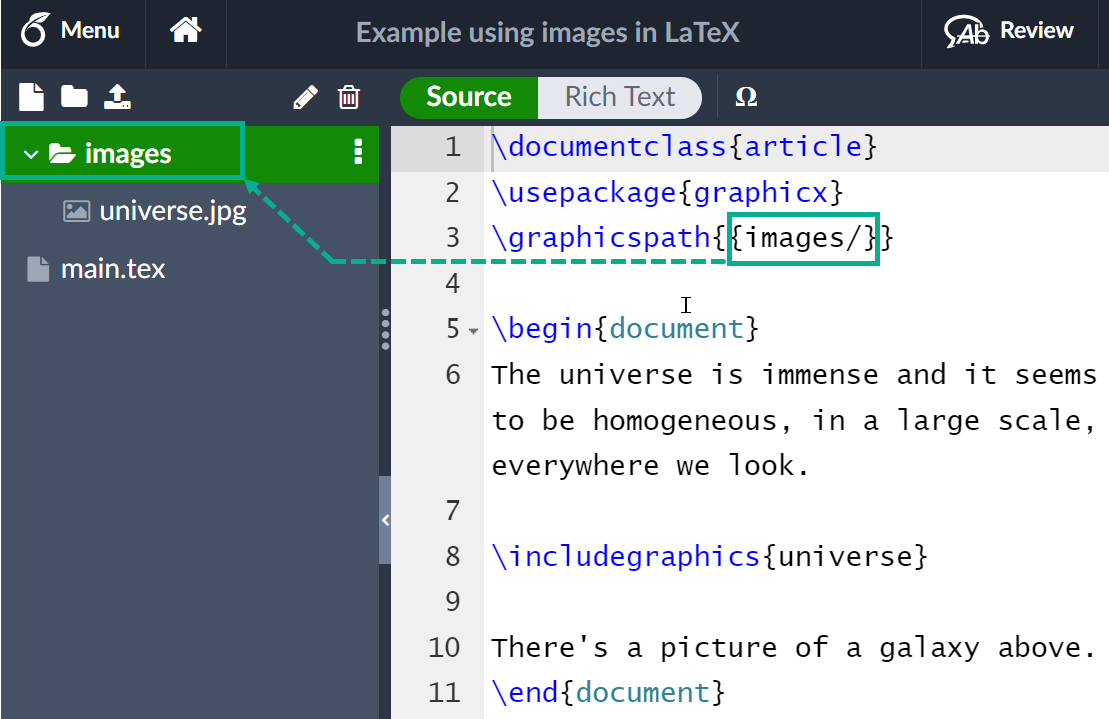
\includegraphics[width=2.75in]{im2.png}\\
\end{figure}

\vspace{1cm}


As a result, SCADA system is covered about 100 km. For
large scale SCADA system it has to set up base stations greater
than one. For mini SCADA it is acceptable. Then, to achieve
the 33 km distance, the power of the customer premises
equipment should be 4 watts effective radiated power relative
to an isotropic source. This system has been defined to enable
users to achieve performance similar to Digital Subscriber Line
(DSL) services. This eventually gives the download speed of
about 1.5 Mbps at the cell edge and an uplink speed of 348
kbps.

\vspace{1cm}\emph{A. \hspace{0.3cm}Communications Topologies}\\
MTU-RTU communication architectures vary among
implementations. The various architectures can be used,
including point-to-point, series, series-star and multi-drop, are
shown in Figure 4. Point-to-point is functionally the simplest
type. However, it is expensive because of the individual
channels needed for each connection. In a series configuration,
the number of channels used is reduced. However, channel
sharing has an impact on the efficiency and complexity of
SCADA operations. Similarly, the series-star and multi-drop
configurations’ use of one channel per device results in
decreased efficiency and increased system complexity. The
four basic architectures shown in Figure 4 can be further
augmented using dedicated communication devices to manage
communication exchange as well as message switching and
buffering. Large SCADA systems, containing hundreds of
RTUs, often employ sub-MTUs to alleviate the burden on the
primary MTU. This type of topology is shown in Figure 5.

\vspace{1cm}


\begin{figure}[h!] % the exclamation point means I REALLY want to honor the [t,h,b] 
  \centering
  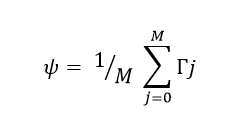
\includegraphics[width=3.5in]{im3.png}\\
\end{figure}

\vspace{1cm}


\vspace{0.2cm}\emph{B. \hspace{0.3cm}Spectrum Sensing}\\
Spectrum sensing, vital part of SCADA communication
system using IEEE 802.22, involves observing the radio
frequency spectrum and processing the observations to
determine if a channel is occupied by a licensed transmission.
Spectrum sensing is included as a compulsory feature within
IEEE 802.22. In IEEE 802.22 both the base station and
equipment sense the spectrum for three different licensed
transmissions such as analog television, digital television and
licensed low power auxiliary devices.

\vspace{1cm}
\subsection{Tabular Data Enter:}

\begin{center}
\begin{tabular}{ |c|c|c|c| } 

\hline

\textbf{Sr no.   }&
\textbf{Roll no.   }&
\textbf{Marks }&
\textbf{Grades  }\\


 \hline
 1  &  101  &  86 & B \\
2  &  102  & 95 & A+ \\
3  &  103  &  93  & A+ \\
4  &  104  &  90  & A \\

 \hline
\end{tabular}
\end{center}
\end{table

\vspace{0.2cm}\emph{C. \hspace{0.3cm}Air Interface}\\
The evident and most critical requirement for the IEEE
802.22 air interface is flexibility and adaptability, since IEEE
802.22 operates in a spectrum where incumbents have to be
protected by all means. Also, because the standard operation is
unlicensed and a base station serves a large area, coexistence
amongst collocated IEEE 802.22 cells is of paramount
importance.

\vspace{1cm}


\begin{figure}[h!] % the exclamation point means I REALLY want to honor the [t,h,b] 
  \centering
  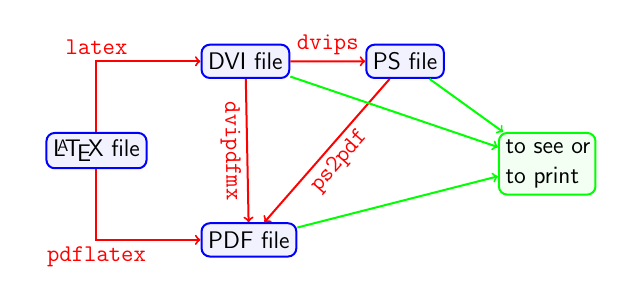
\includegraphics[width=3.5in]{im4.png}\\
\end{figure}

\vspace{1cm}


\emph{D. \hspace{0.3cm}The Physical and Medium Access Control Layer}\\
The PHY layer maintains a high degree of flexibility for
meeting the system requirements [4]. The first characteristic is
the modulation type. An OFDM system has been adopted
because of the resistance against multi-path propagation and
selective fading. Further, the system provides high level of
spectrum efficiency and sufficient data throughput. To provide
access for multiple users, OFDMA is used for both upstream
and downstream data links. IEEE 802.22 allows a variety of
modulation schemes to be used within the OFDMA signal such
as QPSK, 16-QAM and 64-QAM can all be selected with
convolution coding rates of 1/2, 3/4 and 2/3. In order to meet
the requirements for the individual users that may be
experiencing very different signal conditions, it is necessary to
dynamically adapt the modulation, bandwidth and coding on a
per SCADA components basis. In order to be able to obtain the
required level of performance, it has been necessary to the
IEEE 802.22 to adopt a system of what is termed “Channel
Bonding”. This is a technique where the IEEE 802.22 system is
able to utilize more than one channel at a time to provide the
required throughput.


\section{Include table from CSV:
 DSY Admitted students}
 
\hrule 
 
 \hrule
 
 \newline
 
				\begin{Center}
					
			
				\begin{tabular}{|c|c|c|}%
					\hline
					\bfseries Name & \bfseries Age & \bfseries College
					\csvreader[head to column names]{Book1.csv}{}
					{\\\hline\csvcoli&\csvcolii&\csvcoliii}\\
					\hline
				\end{tabular}	
				\end{Center}	

\vspace{1cm}

\vspace{0.2cm}\emph{E. \hspace{0.3cm}Duel-Radio for Real-Time Dedicated Communication}\\
Some questions are arrived like possibility of real-time
dedicated and secured communication in SCADA’s
communication system using IEEE 802.22 as SCADA needs
dedicated secured communication as well as real time. We can
use two different architectures for communication purposes
likes’ primary radio and secondary radio. The primary radio
can provide the wide area coverage due to good propagation of
TV bands and in situation where there is more white space
available in TV bands and/or the TV user density is small, it
can effectively provide broadband access. Again for higher
customer density and capacity requirements, availability of
unused TV bands is low, can be called secondary radio for
transmitting non-critical data, providing as a backup, security
purposes or special circumstances. For both primary radio and
secondary radio the real-time critical data transmission or
emergency data transmission are difficult because of inherent
sensing delays and cognitive nature defined IEEE 802.22.
Therefore, for solution, we can use duel-radio architecture for
secured real-time data transmission in SCADA where one radio
chain is dedicated for data transmission and while the other is
dedicated for spectrum sensing and here, the sensing radio
constantly searches the availability of new channels, as a result,
the other radio chain does not need to delay for data
communication to search the unused bandwidth. Using this
duel-radio architecture can offer high spectrum efficiency and
accurate sensing than single radio architecture that need a small
amount of time slot for spectrum sensing.

\vspace{1cm}


\vspace{0.2cm}\emph{F. \hspace{0.3cm}Scopes to Enhance the Performance}\\
There are several scopes for enhancing the performance of
cognitive radio based IEEE 802.22 standard [6] based
SCADA’s communication for power system. Here we describe
three scopes only. First of all, we know the Base Station’s
coverage area of IEEE 802.22 standard is larger than other
IEEE 802 based standards for example, the range of IEEE
802.16 WiMAX is limited to 5 km. For IEEE 802.22 the Base
Station’s coverage is 33 km during the power level of the
equipments being 4 Watts Effective/Equivalent Isotropic
Radiated Power (EIRP). If higher levels of power are allowed,
this coverage area can be extended to 100 km, as a result, for
wide area coverage the requirements of Base Stations being
lesser. Secondly, the Cognitive Radio Systems can be
implemented using re-configurable and re-programmable
Software Defined Radio (SDR) technology for more flexibility,
therefore, modifications through software upgrades are being
easy. Thirdly, we think for duel radio communications have a
soft limit of capacity because of it’s opportunistically and
dynamically usage of availability of TV channels for increasing
the capacity of the system. To provide SCADA system
components with a level of performance related to Digital
Subscriber Line (DSL) broadband connections a total data rates
of 18 Mbps in a 6 MHz TV channel defined by IEEE 802.22.
For increasing the data rates up to 24 Mbps, the IEEE 802.22
physical layer has to utilize channel bonding and use more than
one TV channels for transmitting and receiving purposes.

\vspace{1cm}

\vspace{0.2cm}\emph{G. \hspace{0.3cm}Comparative Study}\\
SCADA system’s communication can be designed by using
modern cellular communication systems like GSM/GPRS [7],
CDMA [7-10], 3G UMTS [11], IEEE 802.22 WiMAX [12],
satellite based [13] and [14] etc. A comparison of
characteristics of wireless technologies for SCADA system is
given in table 2. From this study we can say that IEEE 802.22
is suitable for future SCADA system’s communication for
future distributed system.

\vspace{1cm}

\vspace{0.2cm}\emph{H. \hspace{0.3cm}Issues, Challenges and Future Study}\\
There are a lot of threats [15] of SCADA system using
IEEE 802.22 standard likes jamming of the channel used to
distribute cognitive messages [16], malicious alteration of
cognitive messages [17], masquerading of a primary user [18],
malicious alteration of a cognitive radio node [17], internal
failure of a cognitive radio node [19], masquerading of a
cognitive radio node [17], hidden node problem [18]
unauthorized use of spectrum bands for DoS to primary users
[16], disruption to the MAC of the cognitive radio network
[21], unauthorized use of spectrum bands for DoS to primary
users [16], saturation of the cognitive control channel [22] and
so on. Although IEEE 802.22 based wireless networks are
promising, there are still problems and difficulties in building it
such as avoiding interference to primary networks, performing
collaborated spectrum sensing among secondary users,
establishing links between secondary users, routing among
secondary users dynamically, improving the throughput of the
entire secondary networks, difficulties on the node
implementation include but not limit to system design,
synchronization among the whole networks, collaboration and
participation among hardware, firmware and software,
algorithm optimization, data conversion from floating point to
fixed point, firmware or software architecture, code
optimization for real-time implementation, system debugging.
All of the above questions and issues need to be answered in
the future research.

\vspace{1cm}

\section{Design for Distribution Monitoring and Control}
In this section we show a design for distribution monitoring
and control for large scale based on IEEE 8022.22. Figure 6
shows an example of a SCADA system implementation. This
particular SCADA system consists of a primary control center
and three field sites. A second backup control center provides
redundancy in the event of a primary control center
malfunction. Point-to-point connections are used for all control
centers to field site communications, with two connections
using radio telemetry. The third field site is local to the control
center and uses the WRAN for communications. A regional
control center sits above the primary control center for a higher
level of supervisory control. The corporate network has access
to all control centers through the WRAN and field sites can be
accessed remotely for troubleshooting and maintenance
operations. The primary control center polls field devices for
data at defined intervals (e.g., 5 seconds, 60 seconds etc.) and
can send new set points to a field device as required. In
addition to polling and issuing high-level commands, the
SCADA server also watches for priority interrupts coming
from field site alarm systems.


\vspace{1cm}

\begin{figure}[h!] % the exclamation point means I REALLY want to honor the [t,h,b] 
  \centering
  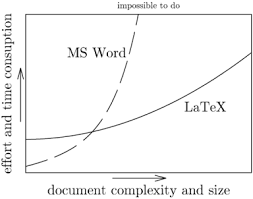
\includegraphics[width=3.5in]{im5.png}\\
\end{figure}

\vspace{1cm}

\section{Design for Railway System Monitoring and Control}
In this section we have shown a design for distribution
monitoring and control for large scale based on IEEE 802.22.
Figure 7 shows an example implementation for rail monitoring
and controlling. This example includes a rail control center that
houses the SCADA system and three sections of a rail system.
The SCADA system polls the rail sections for information such
as the status of the trains, signal systems, traction electrification
systems and ticket vending machines. This information is also
fed to operator consoles within the rail control center. The
SCADA system also monitors operator inputs at the rail control
center and disperses high level operator commands to the rail
section components. In addition, the SCADA system monitors
conditions at the individual rail sections and issues commands
based on these conditions e.g. shut down a train to prevent it
from entering an area that has been determined to be flooded
based on condition monitoring. 

\section{Conclusion}
A SCADA system is a communication and control system
widely used for monitoring, operation and maintenance of
energy infrastructure grids, industries etc. This SCADA system
we can also use in power system using IEEE 802.22 standard
[]. 


\begin{thebibliography} {}

\bibitem {aa}Shubhankar Gawari.,Rucha Kardile.,Stock Price Predictions using Crossover SMA,978-1-6654-1703-7/21.

\bibitem{trishna} Shubhankar Gawari.,Rucha Kardile.,Stock Price Predictions using Crossover SMA,978-1-6654-1703-7/21.

\bibitem{pqr} PQR,Latex ,IEEE

\bibitem{sachi} Sachi Nandan Mohanty.,Rucha Kardile.,Stock Price Predictions using Crossover SMA,978-1-6654-1703-7/21.

\bibitem{rucha} Shubhankar Gawari.,Sachi Nandan Mohanty.,Stock Price Predictions using Crossover SMA,978-1-6654-1703-7/21.

\bibitem{abc} ABC,Research Paper,2022,IEEE.



\end{thebibliography}

\subsection*{Acknowledgements}

Thank You 





\end{document}